\begin{center}
    \begin{figure}[H]
        \centering

        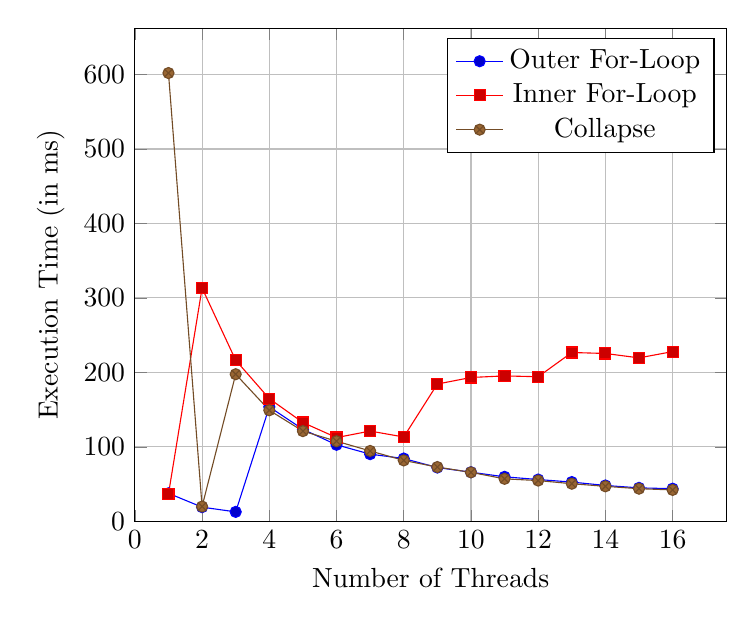
\begin{tikzpicture}
            \begin{axis}[
                title={},
                width=0.75\textwidth,
                xlabel={Number of Threads},
                ylabel={Execution Time (in ms)},
                xmin=0,
                ymin=0,
                grid=major
            ]
                \addplot coordinates {
                    (1,37.6192)(2,19.0143)(3,12.6701)(4,153.6)(5,123.528)(6,102.743)(7,90.193)(8,84.3286)(9,72.2025)(10,65.9573)(11,59.7616)(12,56.1131)(13,52.7063)(14,48.1298)(15,44.9207)(16,43.8277)
                };
                \addlegendentry{Outer For-Loop}

                \addplot coordinates {
                    (1,36.5978)(2,313.246)(3,216.304)(4,164.724)(5,132.658)(6,112.436)(7,121.197)(8,113.254)(9,184.333)(10,193.15)(11,195.278)(12,194.14)(13,226.703)(14,225.382)(15,219.47)(16,227.906)
                };
                \addlegendentry{Inner For-Loop}       

                \addplot coordinates {
                    (1,601.954)(2,19.8608)(3,197.528)(4,149.097)(5,121.117)(6,107.558)(7,94.5198)(8,81.7579)(9,72.864)(10,65.7456)(11,57.0341)(12,54.7264)(13,50.4797)(14,46.9844)(15,43.8079)(16,42.1596)
                };
                \addlegendentry{Collapse}
            \end{axis}
        \end{tikzpicture}
        \caption{Emboss Performance Tests dice.png}
    \end{figure}
\end{center}